The Discontinuous Galerkin method results in truncation error that scales as $h^{N+1}$, where $h$ is the element size and $N$ is the order of the interpolating polynomials within the element.~\cite{dghesthaven} The radial self force is given by the radial derivative of the scalar field, $F_r=\partial_r\Psi$. However, to obtain this quantity, it is necessary to sum the radial derivatives over all $l$ and $m$ modes. Let $F_l=\sum_{m=-l}^l F_{lm}$. Each of these modes, separately, follows the DG convergence scaling laws. It should be possible to extrapolate to infinite DG order based and obtain $F_{\inf}$, the self force for a given l-mode at infinite DG order.

The Lagrange interpolating polynomials that are used as the basis for the Discontinuous Galerkin method may also be used for extrapolation. Consider the case of a three degrees of freedom, for a quadratic polynomial. If $y_i=f(x_i)$ for $i=0-2$~\cite{NRinC++},
\begin{eqnarray}
P(x)=&\frac{(x-x_1)(x-x_2)}{(x_0-x_1)(x_0-x_2)}y_0\nonumber\\
&+\frac{(x-x_0)(x-x_2)}{(x_1-x_0)(x_1-x_2)}y_1\nonumber\\
&+\frac{(x-x_0)(x-x_1)}{(x_2-x_0)(x_2-x_1)}y_2
\end{eqnarray}
However, this form of extrapolation is insufficient for the case of a function that is fundamentally exponential in form. Nowhere does it approximate a polynomail. It is necessary to extend the extrapolation to one based upon exponential, rather than polynomial, assumptions about the underlying functional form.

The three-point exponential extrapolation is motivated by our assumption that Discontinuous Galerkin error is one-sided in the truncation error regime-- it is not random; hence, the self force more or less monotonically approaches a limit. In the round-off error regime where the error is random, the self-force is no longer monotonically decaying. As long as it is monotonically decaying, it can be written in the form of $F_r(n,l)=F_\infty(l)+c(l)\exp[-\alpha n]$, where $n$ is the DG order. For a given mode, the three-point extrapolation is given by
\begin{eqnarray}
h=&\frac{F_r(n_1,l)-F_r(n_2,l)}{F_r(n_1,l)-F_r(n_3,l)}\\
g(\alpha)=&\frac{\exp[\alpha(n_1-n_2)]-1}{-1+\exp[\alpha(n_1-n_3)]}\\
g(\alpha)-h=&0\\
c(l)=&\frac{F_r(n_1)-F_r(n_2)}{\exp[-\alpha n_1]-\exp[-\alpha n_2]}\\
F_\infty(l)=&F_r(n_3)-c(l)\exp[-\alpha n_3]
\end{eqnarray}
In the middle step, it is necessary to use the bisection method for root finding, numerically, with the condition that $\alpha$ may never be less than zero since the solution must decay. If the three points are not monotonic, sometimes there is not a solution. I use extrapolation starting orders from the set 12, 16, 20, 24, 28, 32, and 36, with additional data at orders 40 and 44 that may be used as points two and three in the extrapolation. Figure~\ref{galpha} shows the form of $g(\alpha)$. From this plot, it is clear why $h$ must be greater than $0.5$ in order for $g(\alpha)-h$ to have a root. 


\begin{figure}
  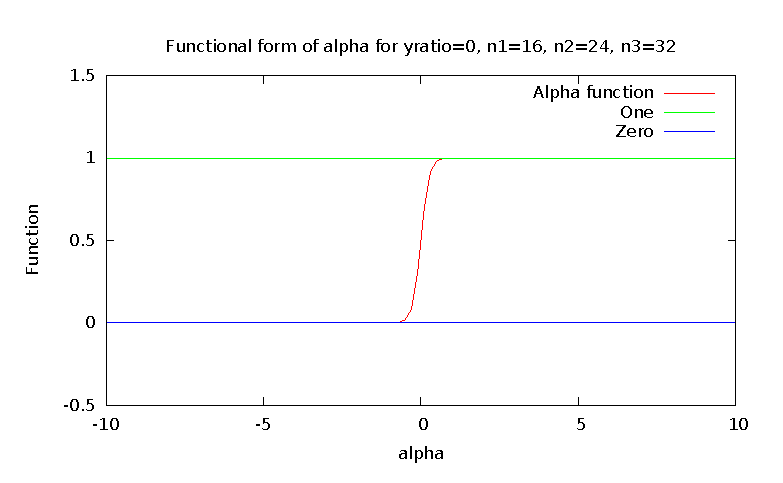
\includegraphics{alphafunction}
  \caption{$g(\alpha)$, $h$ must be greater than $0.5$ for the mode and starting order to have a solution at that specific time.}
  \label{galpha}
\end{figure}



Since some modes fail, it is not possible to chose the same starting order for the extrapolation for all modes and all times. The first attempt I made to improve the choice of starting order was to chose the highest starting order for which no lower starting order had been unsolvable. Figure~\ref{finfovertimediscont} shows this approach leads to some discontinuities in the time evolution of $F_{\infty}$ in some l-modes ($l=3$ is shown). 





\begin{figure}
  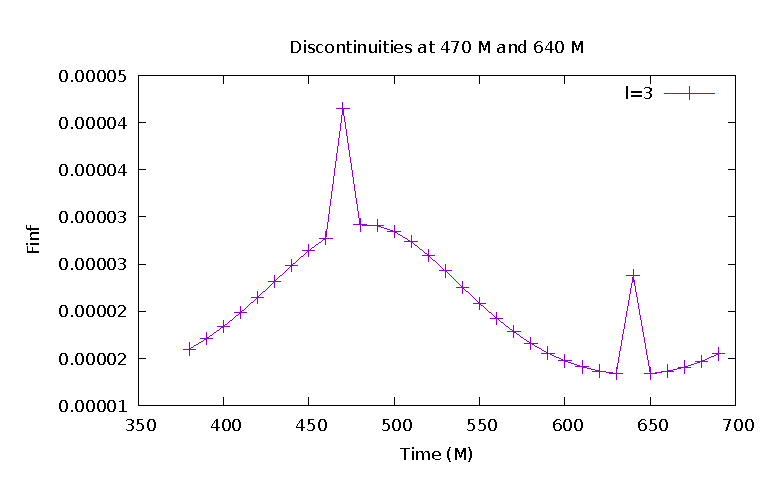
\includegraphics{finfovertimel3discontinuities}
  \caption{Starting order was chosen by iterating from the lowest order to the first order for which the ``mode failed'', and chosing the maximum starting order that succeded. When $F_{\inf}$ is evolved over one full orbital cycle, some l-modes shows discontinuities at some times. l=3}
\label{finfovertimediscont}
\end{figure}

To address this concern, I examined the choice of starting order more closely for specific times where discontinuities were present. One example, for $l=2$ and $t=632M$, is shown in a Table~\ref{manual}. Figure~\ref{nosoln} shows an example where no solution is found. The roundoff noise is visible in Figure~\ref{roundoff} at high DG orders. In Figure~\ref{offset}, it is possible the effect at high DG orders is roundoff noise in the $F_r(n,l)$ values of the points, but it is more likely that it is roundoff noise in the choice of $F_\infty$ due to limitations of the root finding method, resulfing in an incorrect offset of the curve. Figure~\ref{manualfix} shows that after selecting an average of the reasonably similar values from Table~\ref{manual}, the discontinuity in the $l=2$ $t=632M$ radial self-force becomes smooth. 


\begin{table}
  \begin{tabular}{ll}
    Starting Order & $F_\infty$\\
    0 & no solution\\
    1 & 2.40975299617e-05\\
    2 & 2.40975300465e-05\\
    3 & 2.40975300114e-05\\
    4 & no solution\\
    5 & 2.40975299291e-05\\
    6 & 2.40975299148e-05\\
  \end{tabular}
  \caption{Manual starting indices and $F_{\inf}$ values for t=632, l=2.}
  \label{manual}
\end{table}

\begin{figure}
  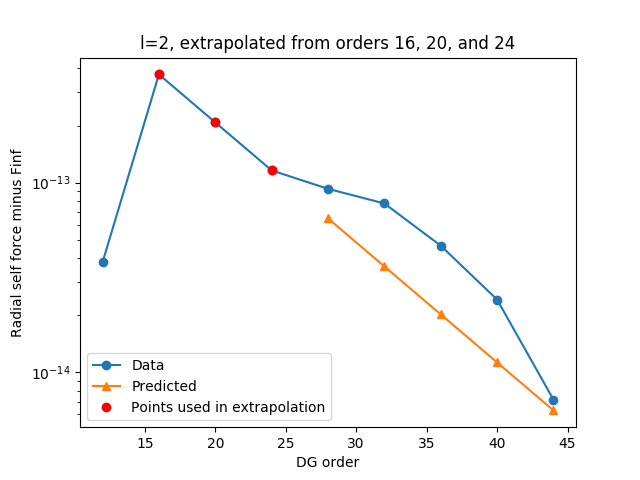
\includegraphics{extrapolate7t632l2i1}
  \caption{Fluctuation in one of the points chosen in the extrapolation, due to roundoff or truncation error, causes the extrapolation to predict a value of $F_{\inf}$ that is subtly wrong, leading to curvature in the semilog plot after $F_{\inf}$ subtraction. t=632, l=2, i=1}
  \label{nosoln}
\end{figure}

\begin{figure}
  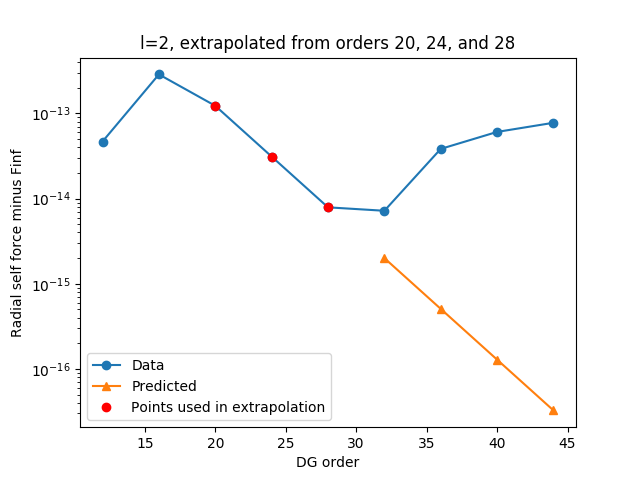
\includegraphics{extrapolate7t632l2i2}
  \caption{Roundoff error is visible at high DG orders. t=632, l=2, i=2}
  \label{roundoff}
\end{figure}

\begin{figure}
  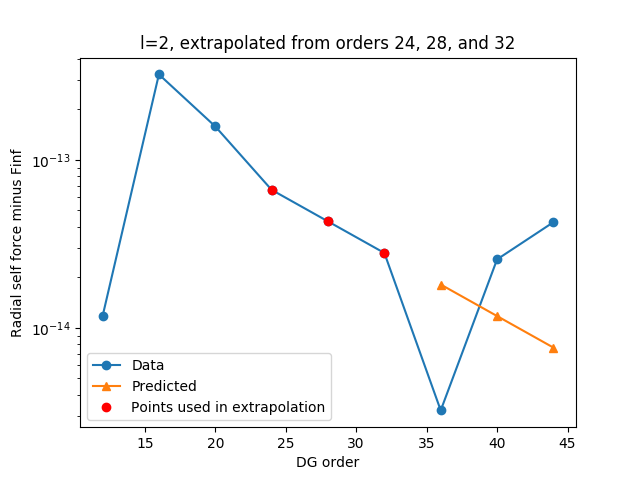
\includegraphics{extrapolate7t632l2i3}
  \caption{The incorrect value of $F_{\inf}$ has been chosen due to roundoff error, perhaps due to finite precision in the root finding algorithm, leading to a negative values, that show as a ``V'' in the semilog plot. t=632, l=3, i=3}
  \label{offset}
\end{figure}


\begin{figure}
  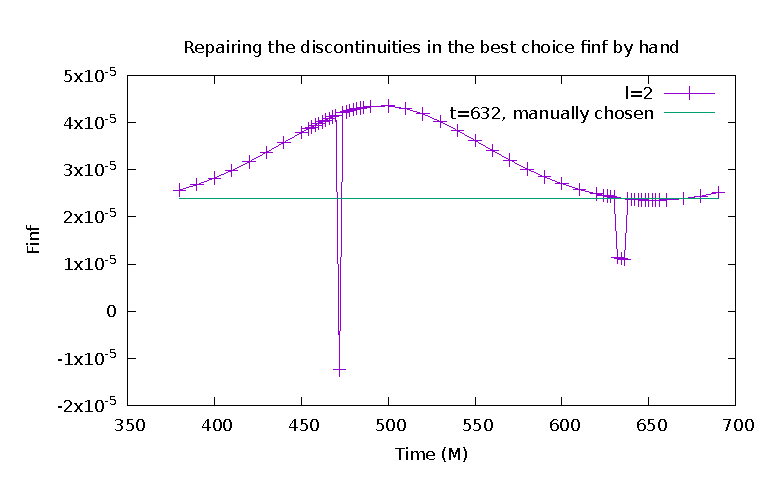
\includegraphics{bestFinfManuallyChosent632l2}
\caption{Manual correction for the discontinuities in the l=2 mode, using the manually determined $F_{\inf}$ data from Table~\ref{manual}. }
\label{manualfix}          
\end{figure}

\subsection{ Checking for discontinuities in $F_{\inf}$ for each each l-mode}

In the median approach, the starting orders that had a solution at each time and for each mode are ordered by their $F_{\inf}$ values. The median value of $F_{\inf}$ is selected, presumably discarding those effected by roundoff and those effected by failure to converge. However, there is no guarantee that it selects those in this regime, since in principle a mode could both be in the roundoff limit and have not converged yet. Yet when this is done, there are no discontinuities in $F_{\inf}$ for any of the l-modes when the median approach is used. See mode zero for an example. The maximum or the minimum may also be chosen.

\begin{figure}
  \includegraphics{finfovertimel0}
  \caption{An example of no discontinuities in $F_{\inf}$ for any of the l-modes. Mode $l=0$.}
\end{figure}


\subsection{Determining $F_{\inf}$ using maximum likelihood fits to subsegments of lines in semilog space}
A better motivated approach, is to fit subsegments of lines in semilog space onthe DG order convergence plot, and find the most linear, longest linear, region. A fit with the ``best'' value of the reduced chi squared should be a good approximation to this. The reduced chi squared is the value of the sum of the residuals of the fit squared divided by the number of degrees of freedom, which in this case is the number of points in the fit minus two, since there are two degrees of freedom in a linear fit. The expectation value of the reduced chi squared, in the limit of a large number of degrees of freedom, is one. I loop over starting and ending points of the fit, and over starting orders, and choose the starting order with the best fit line segment in the sense that that line segment has a reduced chi squared closest to one. An example of such an automatically chosen starting index is given in Figure~\ref{autoconverge}, where there is a long exponentially converging region. Figure~\ref{abserrfitmedian} shows that the absolute error between fit and median techniques increases with l-mode, possibly indicating that roundoff error becomes a more significant factor in the median technique as the l-mode increases, and the fit technique becomes more important.

\begin{figure}
  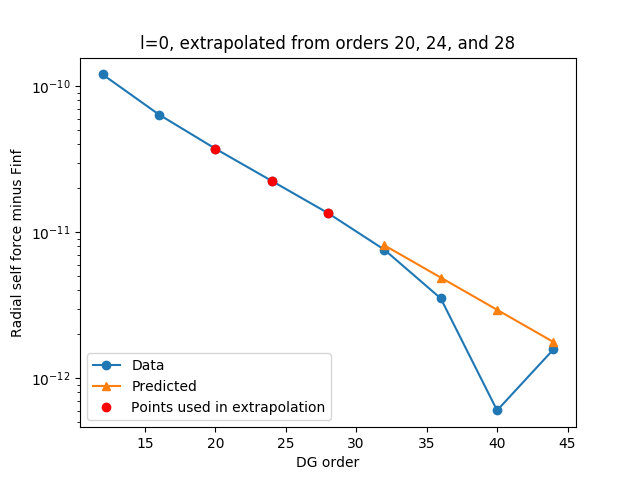
\includegraphics{fittingtechniqet370l0}
  \caption{l=0 mode with line-segment fit-chosen starting order produces convergence plot with long exponentially converging region}
\end{figure}


\begin{figure}
  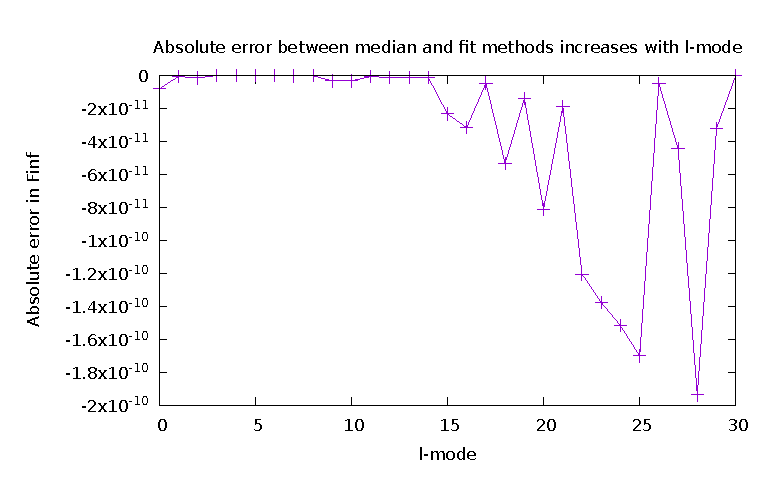
\includegraphics{absErrorIncreaseslmode}
  \caption{Absolute error between fit and median techniques increases with l-mode.}
\end{figure}




